\section{Meetings for the project}



\begin{flushleft}
	\begin{tabular}{l l l l}
		
		{\Large \textbf{Date:}}	& October 16, 2017 & &\\
		{\Large \textbf{Reunion \#: }} & 1 & & \\ 
		{\Large \textbf{Place: }} & LF2L & &\\ % Partner names
		{\Large \textbf{Présents : }}	& \tabitem Fabio Cruz & \tabitem Mauricio Camargo & \tabitem Hakim Boudaoud\\		
	\end{tabular}
\end{flushleft}


\subsubsection*{Goal of the meeting FabCities} 
To establish a the first elements to consider for the \textbf{``Printability Index''}.
\begin{enumerate}[noitemsep]
	\item Definition of the elements of the \textit{Printability Index}
	\item Establishement of possible projects.
\end{enumerate}


\subsubsection*{Discussion/ Comments / Questions} 

First proposition of a "\textit{Printability Index}" is presented in the figure \ref{Printability.Index}:

%\begin{figure}[H]
%	\centering
%	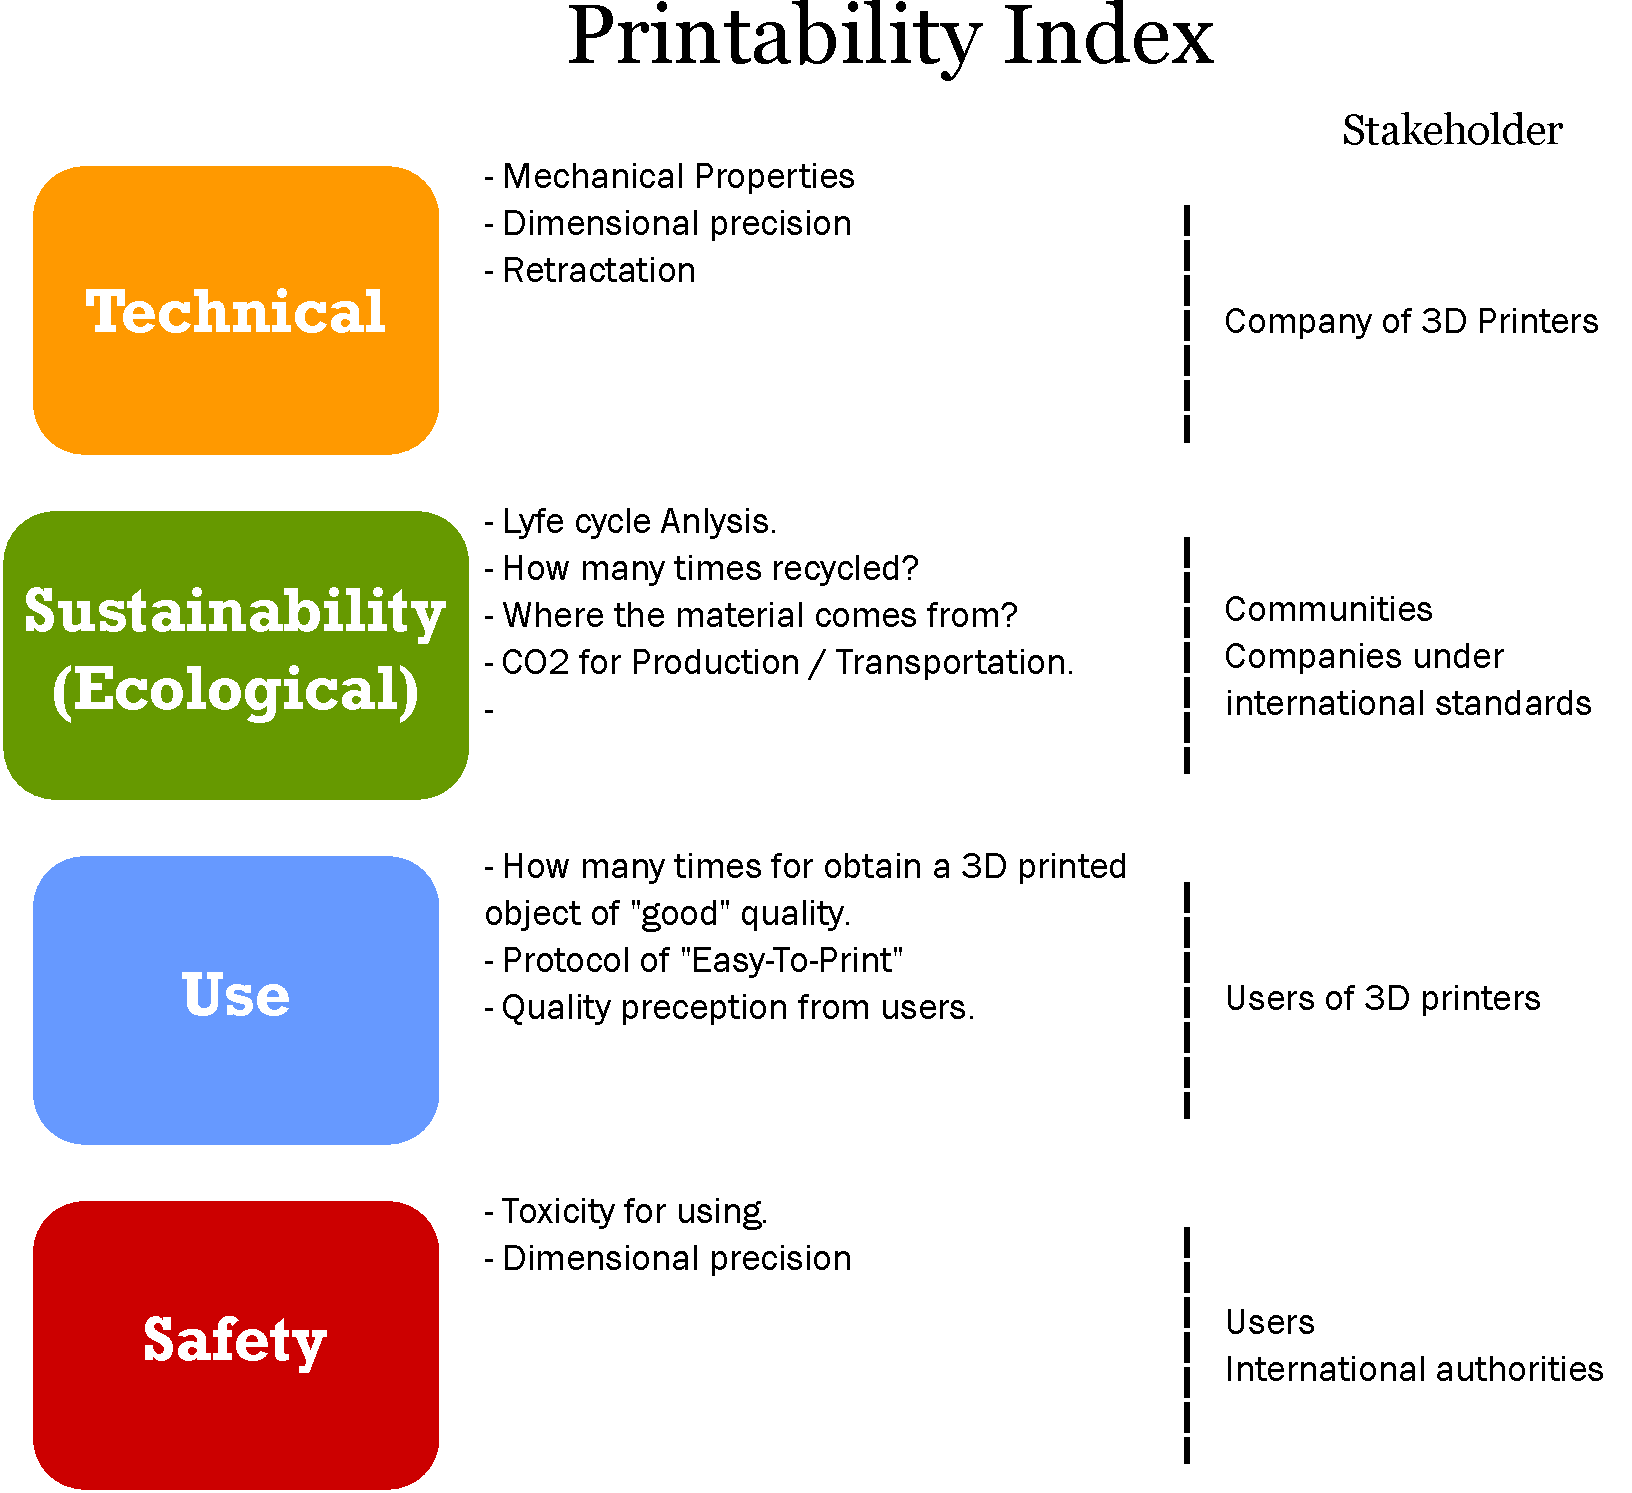
\includegraphics[width=0.6\textwidth]{Figures/Printability-Index/Methodology.pdf}
%	\caption{Four materials from Broplast Association}
%	\label{Printability.Index}
%\end{figure}

\begin{enumerate}[noitemsep]
	\item Elements to consider in the printability index
	\begin{itemize}
		\item Index based in aggregation criteria taking into account the different type of data (e.g. Quantitive, Quality, Statistical)
		\item The index qualifies the \textbf{Filament}. Not the extrusion or recycling process.
		\item This index is intended to qualify the whole chain of printing and in function of different stakeholders.
		\item Article for each axis of the index.
		
	\end{itemize}
\end{enumerate}


\subsubsection*{Possible Projects}

\begin{enumerate}[noitemsep]
	\item Simplification of the protocol and benchmarking model to evaluate the dimensional precision of the machine. Possible research question to start:
	
	\begin{itemize}
		\item How to evaluate the degree of sustainability and dimensional precision of a material for fused filament fabrication process in the green fablab framework \footnote{Comment évaluer le degrée de durabilité et de precision d’impression d’un filament dans le cadre d’un Green FabLab.}.
		\item Protocol design for evaluating 
	\end{itemize}
	
	\item \textbf{Technical aspects:}
	
	\begin{itemize}
		\item Recycle using the extrusion process at LF2L to evaluate mechanical properties
		\item Dimensional precision of using virgin and recycled material.
	\end{itemize}
	
	\item \textbf{Sustainability aspects:}
	
	\begin{itemize}
		\item Protocol and reading grid for the suppliers of filament in order to know the origin of the material, $CO_{2}$ impact. (Pavlo's thesis?)
		\item Dynamical database to have a profile of the suppliers.
	\end{itemize}
	
	\item \textbf{Use aspects:}
	
	\begin{itemize}
		\item Protocol to evaluate the "Easy-to Print".
		\item Evolution of the quality (e.g aesthetics?, color degradation?) of the printed object using recycled material.
		\item Reliability of printing using different types of machines.
	\end{itemize}
	
	\item \textbf{Safety aspects::}
	
	\begin{itemize}
		\item Toxicity protocol. (LIST - Sebastian Zinck)
		
	\end{itemize}
	
\end{enumerate}

%\section*{Date of the Next Meeting} 
%
%\textcolor{blue}{\textbf{Friday 29, 2017 14h at LF2L}}